\section{Introdução: Cinemática tridimensional de corpos rígidos}
\label{sec:introducao}

A cinemática é a parte da mecânica que estuda o movimento dos corpos, sem se preocupar com as causas que o provocam. A cinemática tridimensional de corpos rígidos é um ramo da cinemática que estuda o movimento de corpos rígidos em três dimensões. Corpos rígidos são corpos que não deformam, ou seja, a distância entre dois pontos quaisquer do corpo é constante. A cinemática tridimensional de corpos rígidos é uma área de estudo importante para a engenharia, pois permite a análise de movimentos de corpos rígidos em três dimensões, o que é essencial para o projeto de máquinas e equipamentos.

\subsection{Aplicações da cinemática}
\label{sec:aplicacoes}

As aplicações passam por diversas ferramentas, como sistemas de transmissão, acionamentos mecânicos, automatização de movimentos repetitivos, processos, robótica, entre outros.
Trata-se de uma forma de planejar e controlar o funcionamento de máquinas e equipamentos, criando as bases para a especificação de materiais, dimensionamento de componentes, seleção de motores e atuadores, entre outros.

\begin{figure}[h]
    \centering
    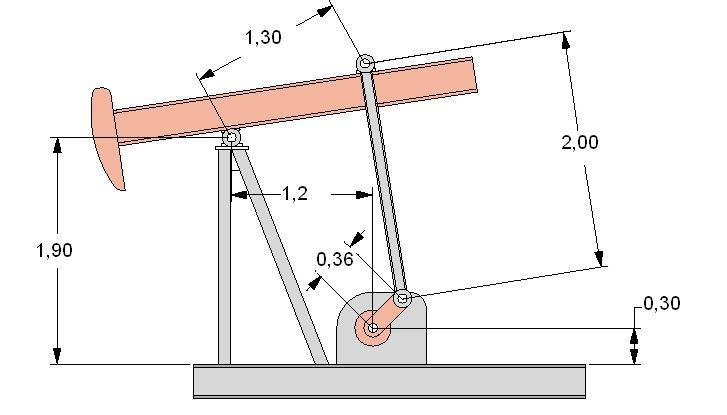
\includegraphics[width=0.9\textwidth]{images/mec4barras}
    \caption{Exemplo de mecanismo de quatro barras utilizado em bombas de extração de petróleo.}
    \label{fig:mec4barras}
\end{figure}


\section{Conceitos Fundamentais}
\label{sec:conceitos}

Para a cinemática, o entendimento de rotação e translação é fundamental para descrever o comportamento dos corpos.

A rotação, em um sistema 3D é descrita por um vetor de rotação, que é um vetor unitário que indica o eixo de rotação e o sentido da rotação. A magnitude do vetor de rotação é o ângulo de rotação. A rotação de um corpo rígido em torno de um eixo é descrita por um ângulo de rotação e um vetor de rotação.

\begin{figure}[H]
    \centering
    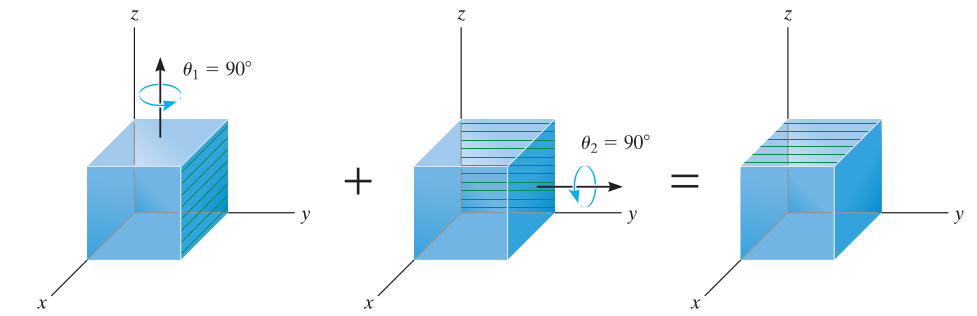
\includegraphics[width=0.9\textwidth]{images/rotacoes}
    \caption{Exemplo de rotação de um corpo rígido em torno de um eixo.}
    \label{fig:rotacao}
\end{figure}

A translação é o movimento de um corpo rígido em que todos os pontos do corpo se movem na mesma direção e sentido. A translação de um corpo rígido é descrita por um vetor de translação, que é um vetor que indica a direção e o sentido do movimento. A magnitude do vetor de translação é a distância percorrida pelo corpo.